

% 1 : x; 2: y; 3: tikz object name
\newcommand\smemRRarb[3]{
    \node[circle, draw, color=black, anchor=south, thick, minimum size=1cm, inner sep=0pt] (#3) at (#1, #2) {A};
    \draw[ultra thick, ->, >=latex] (#3.west) -- ([yshift=-0.6em]#3.west); 
}

% X, Y, PRINTNAME, tikzlabel
\newcommand\smemCore[4]{
    \node[rectangle, draw, color=black, thick, anchor=south west, minimum width=2cm, minimum height=1cm, inner sep=0pt] (#4) at (#1, #2) {#3};
}

% X, Y, PRINTNAME, tikzlabel
\newcommand\smemBank[4]{
    \node[rectangle, draw, color=black, thick, anchor=south west, minimum width=2.5cm, minimum height=1cm, inner sep=0pt] (#4) at (#1, #2) {\emph{#3}};
    \smemRRarb{#1-1}{#2}{arb#4}
    \draw[thick] (arb#4.east) -- (#4.west);
}

% X, Y, tikzlabel
\newcommand\addrSpace[3]{
    \node[rectangle, draw, color=black, thick, anchor=south west, minimum width=2.5cm, minimum height=2cm, inner sep=0pt] (hw#3) at (#1,#2) {{ Phy. addr.}};
    \node[rectangle, draw, color=black, thick, anchor=south west, minimum width=2.5cm, minimum height=2cm, inner sep=0pt] (virt#3) at (#1,#2+2) {{ Virt. addr.}};
    \node[anchor=south west] at (#1,#2) {\small \ttfamily 0x00000 };
    \node[anchor=south west] at (#1,#2+2) {\small \ttfamily 0x20000 };
}


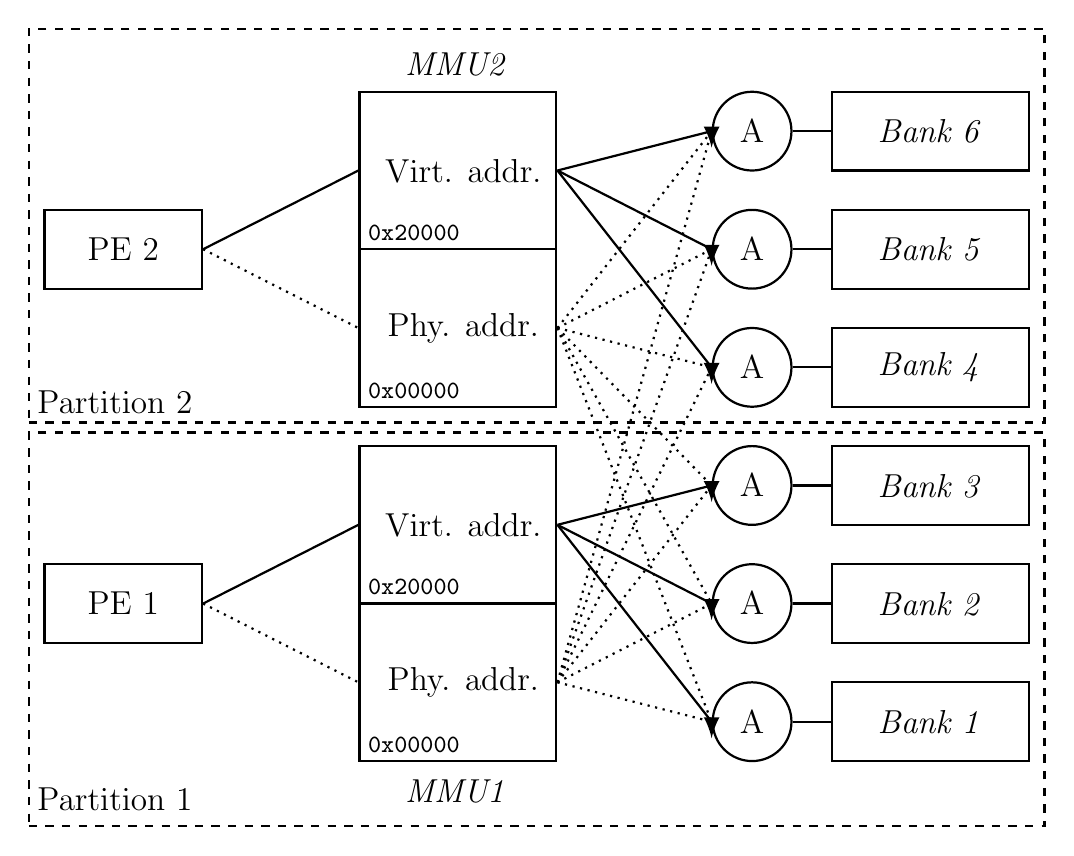
\begin{tikzpicture}[font={\fontsize{12pt}{12}\selectfont}]

    \smemCore{0}{6}{PE 2}{pe2}
    \smemCore{0}{1.5}{PE 1}{pe1}

    \addrSpace{4}{0}{mmu1}
    \node[anchor=north] at (5.25,-0.1) {\emph{MMU1}};
    \addrSpace{4}{4.5}{mmu2}
    \node[anchor=south] at (5.25,8.6) {\emph{MMU2}};
    
    \smemBank{10}{7.5}{Bank 6}{bank6}
    \smemBank{10}{6}{Bank 5}{bank5}
    \smemBank{10}{4.5}{Bank 4}{bank4}
    \smemBank{10}{3}{Bank 3}{bank3}
    \smemBank{10}{1.5}{Bank 2}{bank2}
    \smemBank{10}{0}{Bank 1}{bank1}
    
    \draw[thick, dotted] (pe1.east) -- (hwmmu1.west);
    \draw[thick, dotted] (hwmmu1.east) -- (arbbank1.west);
    \draw[thick, dotted] (hwmmu1.east) -- (arbbank2.west);
    \draw[thick, dotted] (hwmmu1.east) -- (arbbank3.west);
    \draw[thick, dotted] (hwmmu1.east) -- (arbbank4.west);
    \draw[thick, dotted] (hwmmu1.east) -- (arbbank5.west);
    \draw[thick, dotted] (hwmmu1.east) -- (arbbank6.west);
    \draw[thick, dotted] (pe2.east) -- (hwmmu2.west);
    \draw[thick, dotted] (hwmmu2.east) -- (arbbank1.west);
    \draw[thick, dotted] (hwmmu2.east) -- (arbbank2.west);
    \draw[thick, dotted] (hwmmu2.east) -- (arbbank3.west);
    \draw[thick, dotted] (hwmmu2.east) -- (arbbank4.west);
    \draw[thick, dotted] (hwmmu2.east) -- (arbbank5.west);
    \draw[thick, dotted] (hwmmu2.east) -- (arbbank6.west);

    \draw[thick] (pe1.east) -- (virtmmu1.west);
    \draw[thick] (virtmmu1.east) -- (arbbank1.west);
    \draw[thick] (virtmmu1.east) -- (arbbank2.west);
    \draw[thick] (virtmmu1.east) -- (arbbank3.west);
    \draw[thick] (pe2.east) -- (virtmmu2.west);
    \draw[thick] (virtmmu2.east) -- (arbbank4.west);
    \draw[thick] (virtmmu2.east) -- (arbbank5.west);
    \draw[thick] (virtmmu2.east) -- (arbbank6.west);

    \node[draw, rectangle, thick, dashed, anchor=north west, minimum width=12.9cm, minimum height=5cm] at (-0.2,4.2) {};
    \node[draw, rectangle, thick, dashed, anchor=south west, minimum width=12.9cm, minimum height=5cm] at (-0.2,4.3) {};
    \node[anchor=north west] at (-0.2,-0.2) {Partition 1};
    \node[anchor=south west] at (-0.2,4.3) {Partition 2};
\end{tikzpicture}
